% Created 2022-07-06 Wed 13:21
% Intended LaTeX compiler: pdflatex
\documentclass[handout]{beamer}\usepackage{listings}
\usepackage{color}
\usepackage{amsmath}
\usepackage{array}
\usepackage[T1]{fontenc}
\usepackage{natbib}
\lstset{
keywordstyle=\color{blue},
commentstyle=\color{red},stringstyle=\color[rgb]{0,.5,0},
literate={~}{$\sim$}{1},
basicstyle=\ttfamily\small,
columns=fullflexible,
breaklines=true,
breakatwhitespace=false,
numbers=left,
numberstyle=\ttfamily\tiny\color{gray},
stepnumber=1,
numbersep=10pt,
backgroundcolor=\color{white},
tabsize=4,
keepspaces=true,
showspaces=false,
showstringspaces=false,
xleftmargin=.23in,
frame=single,
basewidth={0.5em,0.4em},
}
\usepackage{natbib, dsfont, pgfpages, tikz,amssymb, amsmath,xcolor}
\bibliographystyle{abbrvnat}
% New operators and commands
\newcommand{\Z}{\mathbb{Z}}
\newcommand{\Q}{\mathbb{Q}}
\newcommand{\R}{\mathbb{R}}
\newcommand{\N}{\mathbb{N}}
\newcommand{\C}{\mathbb{C}}
\renewcommand{\S}{\mathbb{S}}
\newcommand{\blank}{\makebox[1ex]{\textbf{$\cdot$}}}
\newcommand\independent{\protect\mathpalette{\protect\independenT}{\perp}}
\def\independenT#1#2{\mathrel{\rlap{$#1#2$}\mkern2mu{#1#2}}}
\renewcommand{\phi}{\varphi}
\renewcommand{\epsilon}{\varepsilon}
\newcommand*\diff{\mathop{}\!\mathrm{d}}
\newcommand{\weakly}{\rightsquigarrow}
\newcommand\smallO{
  \mathchoice
    {{\scriptstyle\mathcal{O}}}% \displaystyle
    {{\scriptstyle\mathcal{O}}}% \textstyle
    {{\scriptscriptstyle\mathcal{O}}}% \scriptstyle
    {\scalebox{.6}{$\scriptscriptstyle\mathcal{O}$}}%\scriptscriptstyle
}
\newcommand{\midd}{\; \middle|\;}
\newcommand{\1}{\mathds{1}}
\usepackage{ifthen} %% Empirical process with default argument
% \newcommand{\G}[1][]{%
%    \ifthenelse{ \equal{#1}{} }
%       {\ensuremath{\mathbb{G}_n}}
%       {\ensuremath{\mathbb{G}_{#1}}}
% }
% New version:
\newcommand{\G}[2][n]{
{\ensuremath{\mathbb{G}_{#1}}{\left[#2\right]}}
}
\DeclareMathOperator*{\argmin}{\arg\!\min}

% New operators for consistent notation
\newcommand{\V}{\mathrm{Var}} % variance
\newcommand{\measure}[1]{\mathrm{{#1}}} % measure
% \newcommand{\measure}[1]{\textnormal{\textbf{{#1}}}} % measure
\newcommand{\m}[1]{\measure{#1}} % measure shortcut
\newcommand{\eqd}{\stackrel{d}{=}} % equality in distribution
\newcommand{\arrow}[1]{\xrightarrow{\; {#1} \;}}
\newcommand{\arrowP}{\xrightarrow{\; \m{P} \;}} % convergence in probability
\newcommand{\leb}{\lambda} % the Lebesgue measure
\newcommand{\T}{\top} % transpose
\newcommand{\KL}{\ensuremath{D_{\mathrm{KL}}}}

\usepackage{xargs}
% Make it easy to change counterfactual notation:
\newcommandx{\cf}[4][3={}, 4={}]{
  % \ifthenelse{ \equal{#4}{} }
  % {{#1^{#2}}(#3)}
  {\ifthenelse{ \equal{#3}{} }
    {{#1^{#2}}_{#4}}
    {{#1^{#2}}_{#4}(#3)}}
}

% Easily change notation:
\DeclareMathOperator{\TT}{\Psi} % target parameter
\newcommand{\lp}{\mathcal{L}_{\P}^2} % shortcut for lp2 space
\newcommand{\empmeas}{\hat{\mathbb{P}}_n} % empirical measure
\DeclareMathOperator{\E}{\mathbb{E}} % expectation
\renewcommand{\P}{\m{P}} % probability
\newcommand{\ic}{\mathrm{IF}} % influence curve
\usepackage[noend,ruled]{algorithm2e}
\setbeamertemplate{footline}[frame number]
\beamertemplatenavigationsymbolsempty
\usepackage{appendixnumberbeamer}
\setbeamercolor{gray}{bg=white!90!black}

\renewcommand*\familydefault{\sfdefault}
\itemsep2pt
\usepackage[utf8]{inputenc}
\usepackage[T1]{fontenc}
\usepackage{graphicx}
\usepackage{longtable}
\usepackage{wrapfig}
\usepackage{rotating}
\usepackage[normalem]{ulem}
\usepackage{amsmath}
\usepackage{amssymb}
\usepackage{capt-of}
\usepackage{hyperref}
\usetheme{default}
\author{Anders Munch (with Thomas G., Helene, and Paul)}
\date{\today}
\title{Debiased Brier score estimation using TMLE}
\begin{document}

\maketitle
\section{Validating risk prediction models}
\label{sec:orgac65f51}
\begin{frame}[label={sec:orgc76fc5a}]{Disclaimer -- unfinished work}
Mostly theory and not so much implementation and ``results''.

\vfill \pause

You have the opportunity to influence the project!
\end{frame}

\begin{frame}[label={sec:orgc6ae93a}]{Validating risk prediction models}
\begin{block}{Full data}
\begin{description}
\item[{\(X \in \R^p\)}] Static covariates measured at baseline (\(t=0\)).

\item[{\(T \in \R_+\)}] Time of event

\item[{\(t \in \R_+\)}] Fixed time horizon

\item[{\(r(t \mid X) \in [0,1]\)}] Risk prediction at time \(t\) given baseline covariates
\end{description}

\pause     
\end{block}
\begin{block}{Risk prediction model}
We assume the risk prediction model \(r\) is fixed (i.e., non-random); for instance, it could have
been fitted on a separate data set. We want to use the data \((X_i, T_i)\), \(i=1,\dots,n\) to
evaluate the performance of \(r\). \pause
\end{block}
\begin{block}{Example}
Is a particular bio-marker relevant for predicting the risk of developing some disease within
the next two years? Is it relevant when other risk factors are measured?
\end{block}
\end{frame}

\begin{frame}[label={sec:org168a868}]{The Brier score}
\begin{description}
\item[{\(Y(t) \in \{0,1\}\)}] Event indicator at time \(t\), i.e., \(Y(t):= \1\{T \leq t\}\)
\end{description}

\vfill \pause

The (average) Brier score of the risk model \(r\) is the (average of the) squared difference
between \(Y(t)\) and the predicted risk according to the model, i.e.,
\begin{equation*}
  \E\left[ 
    \left\{
      Y(t) - r(t \mid X)
    \right\}^2 \right].
\end{equation*}
\pause \vspace{-1cm}

\begin{block}{$\;$}
\begin{columns}
\begin{column}{.45\columnwidth}
\begin{center}
\begin{tabular}{ll}
Benchmark prediction & Brier score\\
\hline
50\% always & 25\%\\
Overall event prob. & See figure\\
Coin toss & 50\%\\
Uniform[0,1] & 33\%\\
\end{tabular}

\end{center}
\end{column}

\begin{column}{0.45\columnwidth}
\begin{figure}[htbp]
\centering
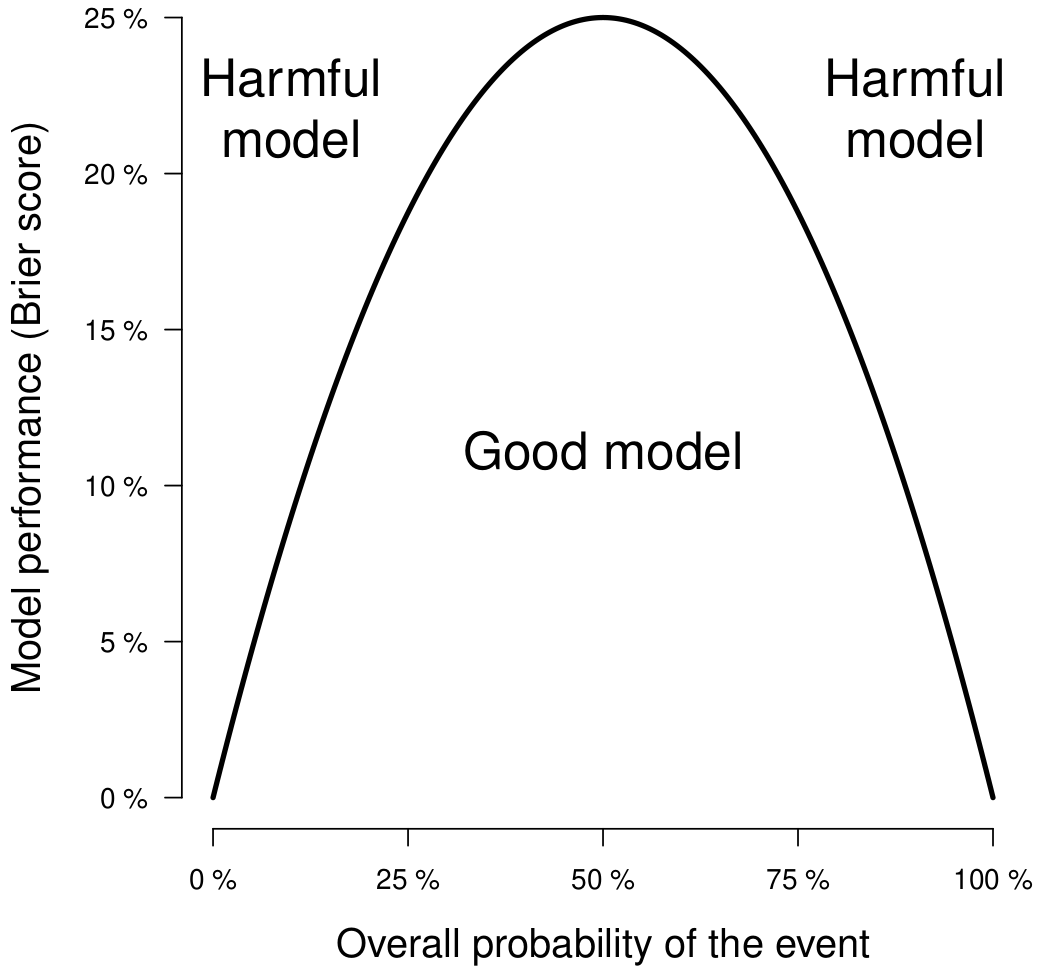
\includegraphics[width=.8\textwidth]{./gerds-kattan-brier-viz.png}
\citep{gerds2021medical}
\end{figure}
\end{column}
\end{columns}
\end{block}
\end{frame}

\begin{frame}[label={sec:org3a8d8e9}]{Obtaining the Brier score from censored data}
In many cases we do not get to observe the event time \(T\). \pause

\begin{block}{Observed data}
\begin{description}
\item[{\(X \in \R^p\)}] Static covariates measured at baseline (\(t=0\)).
\item[{\(\tilde T \in \R_+\)}] Observation time (\(\tilde T := T \wedge C\))
\item[{\(\Delta \in \{0,1\}\)}] Event indicator (\(\Delta := \1\{\tilde T = T\}\))
\end{description}

Let \((X, T) \sim Q\) and \(O := (X, \tilde T, \Delta) \sim P\). \pause
\end{block}

\begin{block}{Inverse probability of censoring weights (IPCW)}
When $T \independent C \mid X$ the Brier score is identifiable from the observed
data\footnote<3->{Note that $W(t)\{Y(t)-r(t\mid X)\}^2$ is a function of the observed data, as
  $Y(t)$ is observed whenever $W(t)$ is non-zero.}:
\begin{equation*}
  \E_Q\left[ 
    \left\{
      Y(t) - r(r \mid X)
    \right\}^2 \right]
  = \E_P\left[
    W(t)
    \left\{
      Y(t) - r(r \mid X)
    \right\}^2 \right],
\end{equation*}
with
\begin{equation*}
  W(t) = \frac{\1({\tilde{T} >t})}{G(t \mid X)} + \frac{\1({\tilde{T}\leq
      t})\Delta}{G(\tilde{T}\mid X)}.
\end{equation*}
\end{block}
\end{frame}


\begin{frame}[label={sec:orgdde99f0}]{Visualizing the reweighting}
\begin{onlyenv}<1>
\begin{center}
\includegraphics[width=.9\linewidth]{/tmp/babel-uSK2rt/figure-63LY1z.pdf}
\end{center}
\end{onlyenv}


\begin{onlyenv}<2>
\begin{center}
\includegraphics[width=.9\linewidth]{/tmp/babel-uSK2rt/figure-hngddQ.pdf}
\end{center}
\end{onlyenv}


\begin{onlyenv}<3>
\begin{center}
\includegraphics[width=.9\linewidth]{/tmp/babel-uSK2rt/figure-Jnvx9e.pdf}
\end{center}
\end{onlyenv}
\end{frame}

\begin{frame}[label={sec:org1f68676}]{Estimating the Brier score from censored data}
\small
By estimating the censoring distribution \(G\) we obtain the IPCW estimator
\begin{equation*}
  \widehat{W}_i(t)=\frac{\1({\tilde{T}_i >t})}{\hat{G}(t \mid X_i)} + \frac{\1({\tilde{T}_i\leq
      t})\Delta_i}{\hat{G}(\tilde{T}_i\mid X_i)},
  \quad \hat{\theta}_n^t = \empmeas[\widehat{W}_i(t)
  \left\{
    Y_i(t) - r(t \mid X_i)
  \right\}^2]
\end{equation*}

\vfill \pause
\begin{itemize}
\item The parametric (\(n^{-1/2}\)) rate of convergence of \(\hat G_n\) is obtainable under suitable
assumptions on the censoring distribution (for instance random censoring or a Cox model),
giving also \(n^{-1/2}\) convergence and asymptotic normality of \(\hat\theta^t_n\). \pause
\item Such assumptions can be unpleasant, in particular if we are validating a risk prediction model
for which we \emph{do not} make similar assumptions (e.g., random forests or other ``data-adaptive''
estimator). \pause
\item When modeling \(G\) with flexible, data-adaptive methods we cannot expect \(n^{-1/2}\)-rate
convergence, and hence the simple plug-in estimator \(\hat\theta^t_n\) cannot be expected to be
\(n^{-1/2}\) consistent and asymptotically normal in this setting. \pause
	 \vfill
\end{itemize}

\begin{beamercolorbox}[rounded=true]{gray}
\normalsize \centering Can we construct an IPCW estimator using ``flexible/data-adaptive''
estimation of G?
\end{beamercolorbox}
\end{frame}

\begin{frame}[label={sec:orge6f3bc6}]{Brier score estimation with ``flexible'' censoring modeling}
By ``flexible'' we mean estimators of the censoring distribution not converging at parametric
(\(n^{-1/2}\)) rate. The problem with the plug-in estimation using such nuisance parameter
estimators is \alert{bias}.
\vfill \pause

\begin{block}{DML \small \citep{chernozhukov2017double} \large / one-step estimation}
Construct estimators as the solution to the empirical efficient score equation. The obtained
estimator is no longer an IPCW estimator. \pause
\end{block}

\begin{block}{Undersmoothing}
Challenging to do for general nuisance parameter estimators, but some recent work for the Highly
Adaptive Lasso (HAL) estimator \small
\citep{ertefaie2020nonparametric,van2019efficient}\normalsize. Seems computationally
challenging. \pause
\end{block}

\begin{block}{TMLE \small \citep{van2011targeted,van2006targeted}}
TMLE constructs a \alert{plug-in estimator} that solves the efficient score equation. Typically based
on the G-formula, but theoretically this should not be important.
\end{block}
\end{frame}

\section{IPCW estimator using TMLE}
\label{sec:org9c5e859}
\begin{frame}[label={sec:orgb63cab9}]{Different ways to the target}
The target parameter (average Brier score) can be identified from the observed data using either
the censoring or the survival distribution as nuisance parameter:
\begin{equation*}
  \E_Q\left[ 
    \left\{
      Y(t) - r(t \mid X)
    \right\}^2 \right]
  = \E_P\left[ \phi^t_{\mathrm{IPCW}}(O; G) \right]
  = \E_P\left[ \phi^t_{\mathrm{alt}}(O; S) \right],
\end{equation*}
with
\begin{equation*}
  \phi^t_{\mathrm{IPCW}}(O; G) = 
  \left(
    \frac{\1({\tilde{T}_i >t})}{G(t \mid X_i)} + \frac{\1({\tilde{T}_i\leq
	t})\Delta_i}{G(\tilde{T}_i\mid X_i)}
  \right) \left\{
    Y(t) - r(t \mid X)
  \right\}^2,
\end{equation*}
and
\begin{equation*}
  \phi^t_{\mathrm{alt}}(O; S) = 
  \left(
    1- S(t \mid X)
  \right) \left\{
    1 - 2r(t \mid X) 
  \right\}  + r(t\mid X)^2.
\end{equation*}
\end{frame}

\begin{frame}[label={sec:org7dbfd63}]{Representations of the efficient influence function}
The functions $\phi^t_{\mathrm{IPCW}}$ and $\phi^t_{\mathrm{alt}}$ are influence functions in
models where, respectively, $G$ or $S$ are known. \pause Semiparametric efficiency theory then
tells us that the efficient influence function $\phi^t$ (under the non-parametric model) can be
obtained as either
\begin{equation*}
  \phi^t = 
  \phi^t_{\mathrm{IPCW}} - \Pi
  \left[
    \phi^t_{\mathrm{IPCW}} \midd \mathcal{T}_{G}
  \right],
\end{equation*}
or
\begin{equation*}
  \phi^t = 
  \phi^t_{\mathrm{alt}} - \Pi
  \left[
    \phi^t_{\mathrm{alt}} \midd \mathcal{T}_{S}
  \right],
\end{equation*}
where $\mathcal{T}_G$ and $\mathcal{T}_S$ are the orthogonal components of the tangent space
corresponding to the parameters $G$ and $S$, i.e., $\mathcal{T} = \mathcal{T}_G \oplus \mathcal{T}_S$.

\vfill \pause

Both representation can be useful; and starting from one, it might not be complete
straightforward to derive the alternative one.
\end{frame}

\begin{frame}[label={sec:org7cde526}]{The efficient influence function}
The two representations give
\begin{align*}
  \phi^t(O; S, G) =   & \phi^t_{\mathrm{IPCW}}(O; G)
  \\ & \quad +
       \{1-r(t \mid X)\}^2 \int_0^t \frac{M^C(\diff s \mid X; G)}{G(s \mid X)}
  \\ & \quad -
       \{1-2r(t \mid X)\} S(t \mid X) \int_0^t \frac{M^C(\diff s \mid X; G)}{G(s \mid X) S(s
       \mid X)},
\end{align*}
and
\begin{align*}
  \phi^t(O; S, G) = & \phi^t_{\mathrm{alt}}(O; S)
  \\ & \quad + \left[ % sign!
    \int_0^t \frac{M(\diff s \mid X; S)}{S(s\mid X)G(s \mid X)} \right] S(t \mid X)
  (1 - 2r(t\mid X)).
\end{align*}
\end{frame}

\begin{frame}[label={sec:org0101e5d}]{Decomposition}
\small
We want to pick the nuisance estimator $\hat G_n$ such that the estimator
\begin{equation*}
  \hat{\theta}^t_n = \tilde{\Psi}^t(\hat G_n, \empmeas) =
  \empmeas
  \left[
    \phi^t_{\mathrm{IPCW}}(O; \hat{G}_n)
  \right]
\end{equation*}
is asymptotically linear (and efficient), i.e., such that
\begin{equation*}
  \hat{\theta}^t_n - \theta = (\empmeas-P)[\phi^t(O;G_P, S_P)] + \smallO_P(n^{-1/2}).
\end{equation*}
\pause Let $f^t:= -\Pi(\phi^t_{\mathrm{IPWC}} \mid \mathcal{T}_G)$ and consider
the decomposition
\begin{align*}
  & \tilde{\Psi}^t(\hat G_n, \empmeas) - \tilde{\Psi}^t(G_P, P)
  \\ & = \empmeas
       \left[
       \phi^t_{\mathrm{IPCW}}(O; \hat{G}_n)
       \right] - \tilde{\Psi}^t(G_P, P)
       \pm \empmeas
       \left[
       f^t(O; \hat{G}_n, \hat{S}_n)
       \right]
  \\ & = \empmeas
       \left[
       \phi^t(O; \hat{G}_n, \hat{S}_n)
       \right] - \tilde{\Psi}^t(G_P, P)
       - \empmeas
       \left[
       f^t(O; \hat{G}_n, \hat{S}_n)
       \right]
  \\ & = (\empmeas-P)
       \left[
       \phi^t(O; \hat{G}_n, \hat{S}_n)
       \right] 
       +\mathrm{Rem}(\hat{G}_n, \hat{S}_n, P)
       - \empmeas
       \left[
       f^t(O; \hat{G}_n, \hat{S}_n)
       \right],
       \\ & =: (A) + (B) + (C)
\end{align*}
with
\begin{equation*}
  \mathrm{Rem}(G, S, P) := P[\phi^t(O ; G, S)] - \tilde{\Psi}^t(G_P, P).
\end{equation*}
\end{frame}

\begin{frame}[label={sec:org6f54abc}]{Donsker condition and remainder term}
\small

Donsker class conditions (or sample splitting) gives
\begin{equation*}
 (A) = (\empmeas-P) \left[ \phi^t(O; \hat{G}_n, \hat{S}_n) \right]
  = (\empmeas-P) \left[ \phi^t(O ; G, S) \right] + \smallO_P(n^{-1/2}).
\end{equation*}

 \vfill \pause

As $\mathrm{Rem}(P, \hat{G}_n, \hat{S}_n) = \tilde{\Psi}^t(\hat{G}_n, P) - \tilde{\Psi}^t(G_P, P) +
P[f^t(O; \hat{G}_n, \hat{S}_n)]$ and $f^t(O; \hat{G}_n, \hat{S}_n)$ acts like the derivative of $G
\mapsto \tilde{\Psi}^t(G, P)$, a functional Taylor expansion would suggest that
\begin{equation*}
  (B) = \mathrm{Rem}(P, \hat{G}_n, \hat{S}_n) = \mathcal{O}_P
  \left(
    \Vert (\hat G_n, \hat S_n) - ( G,  S) \Vert^2
  \right).
\end{equation*}

\vfill \pause   
Thus, when the Donsker condition holds, and $\Vert\hat{G}_n- G\Vert = \smallO_P(n^{-1/4})$ and
$\Vert\hat{S}_n- S\Vert = \smallO_P(n^{-1/4})$, we have
\begin{equation*}
  \tilde{\Psi}^t(\hat G_n, \empmeas) - \tilde{\Psi}^t(G_P, P)
  =  (\empmeas-P)
  \left[
    \phi^t(O; G_P, S_P)
  \right] 
  - \empmeas
  \left[
    f^t(O; \hat{G}_n, \hat{S}_n)
  \right] + \smallO_P(n^{-1/2})
\end{equation*}
\pause TMLE focuses on constructing $\hat{G}_n$ such that
$ (C) = \empmeas \left[ f^t(O; \hat{G}_n, \hat{S}_n) \right] \approx 0$.\footnote<5->{Note that the exact same
  arguments would hold if we replaced $\phi^t_{\mathrm{IPCW}}$ with $\phi^t_{\mathrm{alt}}$ and used
  $f^t=-\Pi(\phi^t_{\mathrm{alt}} \mid \mathcal{T}_S)$ instead of
  $f^t=-\Pi(\phi^t_{\mathrm{IPWC}} \mid \mathcal{T}_G)$.}   
\end{frame}

\begin{frame}[label={sec:org4b6f355}]{The TMLE strategy for controlling the remaining component}
We construct the estimator $\hat{G}$ of $G$ as $\hat{G} = e^{-\hat{\Lambda}_C}$ where
$\hat{\Lambda}_C$ is the cumulative hazard of censoring. \pause We assume available (initial
estimators) $\hat{\Lambda}_C^0$ and $\hat{\Lambda}$, where $\hat{\Lambda}$ is the cumulative
hazard of the event of interest. \pause To construct $\hat{\Lambda}_C$ in the right way, we
recursively construct fluctuation models
\begin{equation*}
  \mathcal{F}^{k}:=
  \left\{
    \hat{\Lambda}_C^{k}(\blank;\epsilon) \, : \, \epsilon \in \R
  \right\} \subset \mathcal{F}, \quad k = 1, 2, \dots, 
\end{equation*}
and let $\epsilon^*_k$ denote the MLE of the fluctuation model $\mathcal{F}^{k}$, and
$\hat{\Lambda}_C^k := \hat{\Lambda}_C^k(\blank; \epsilon^*_k)$ the model corresponding to the MLE. \pause
These should be constructed such that
\begin{enumerate}
\item \label{item:1} At $\epsilon = 0$, $\hat{\Lambda}_C^1(\blank; 0) = \hat{\Lambda}_C^0$ and
  $\hat{\Lambda}_C^{k+1}(\blank;0) = \hat{\Lambda}_C^{k} =
  \hat{\Lambda}_C^{k}(\blank;\epsilon^*_k)$. \pause
\item \label{item:2} The score function of the model
  $\hat{P}_n^{k+1}(\blank;\epsilon)$ equals $f^t$, i.e.,
  \begin{equation*}
    \frac{\partial }{\partial \epsilon} \Big\vert_{\epsilon=0} \log\diff\hat{P}_n^{k+1}(\blank;\epsilon) = f^t(\blank; e^{-\hat{\Lambda}_C^{k}}, e^{-\hat{\Lambda}}).
  \end{equation*}
\end{enumerate}
\end{frame}

\begin{frame}[label={sec:org9bddcde}]{The obtained estimator works}
If the procedure converges after some $K$, we set
$\hat{\Lambda}_C = \hat{\Lambda}_C(\blank \; ; \epsilon^*_K)$; then
\begin{align*}
  \empmeas[f^t(O; e^{-\hat{\Lambda}_C}, e^{-\hat{\Lambda}})]
  & \approx \empmeas[f^t(O; e^{-\hat{\Lambda}_C^{K-1}}, e^{-\hat{\Lambda}})]
  \\ &  = \frac{\partial }{\partial \epsilon} \Big\vert_{\epsilon=0}\empmeas
       \left[
       \log\diff\hat{P}_n^{K}(\blank;\epsilon)
       \right]
  \\ &
       \approx \frac{\partial }{\partial \epsilon} \Big\vert_{\epsilon=\epsilon^*_K}\empmeas
       \left[
       \log\diff\hat{P}_n^{K}(\blank;\epsilon)
       \right]
       = 0,
\end{align*}
as $\epsilon^*_K \approx 0$ because the procedure is converging. 
\end{frame}

\begin{frame}[label={sec:org51b8d19}]{Fluctuation model}
We can choose a multiplicative update step to get the fluctuation model
\begin{equation*}
  \mathcal{F}^{k+1}:=
  \left\{
    \hat{\Lambda}_C^{k+1}(\blank;\epsilon) \midd 
    \hat{\Lambda}_C^{k+1}(\diff s \mid x ; \epsilon) :=  e^{\epsilon g(s, x ;
      \hat{\Lambda}_C^k, \hat{\Lambda} )}  \hat{\Lambda}_C^{k}( \diff s \mid x ),
    \epsilon \in \R
  \right\},
\end{equation*}
where
\begin{equation*}
  g(s, x ; \Lambda_C, \Lambda) :=
  \1(s \leq t)\left\{
    \frac{\{1-r(t \mid x)\}^2}{e^{-\Lambda_C(s \mid x)}}
    - \frac{\{1-2r(t \mid x)\} e^{-\Lambda(t \mid x)}} {e^{-\Lambda_C(s \mid x) - \Lambda(s \mid x)}}
  \right\}.
\end{equation*}
\pause One can then verify that $\hat{\Lambda}_C^{k+1}(\blank;0) = \hat{\Lambda}_C^{k}$ and 
\begin{align*}
  \frac{\partial }{\partial \epsilon} \Big\vert_{\epsilon=0}\log\diff \hat{P}_n^{k+1}(O; \epsilon)
  & = \int g(s, X; \hat{\Lambda}_C^k, \hat{\Lambda})  M_C(\diff s \mid X; \hat{\Lambda}_C)
  \\ & = f^t(O; e^{-\hat{\Lambda}_C^k}, e^{-\hat{\Lambda}}).
\end{align*}
\end{frame}

\begin{frame}[label={sec:org4f71973}]{Final algorithm}
\small
\begin{algorithm}[H]
  \caption{TMLE-based IPCW estimator of the average Brier score.}
  \SetKwInOut{KwIn}{Input}
  \SetKwInOut{KwOut}{Output}

  \KwIn{Data $O_i$, $i=1, \dots, n$, risk prediction model $r$, and estimates $\hat{\Lambda}_C^0$ and $\hat{\Lambda}$}

  \KwOut{Estimate of the average Brier score}
    $\epsilon^* \gets \infty$

  $\hat{\Lambda}_C \gets \hat{\Lambda}_C^0$

  \While{$\epsilon^* \not \approx 0$}{

    $
    g(s, x ; \hat{\Lambda}_C, \hat{\Lambda}) \gets \1(s \leq t)\left\{ \frac{\{1-r(t \mid x)\}^2}{e^{-\hat{\Lambda}_C(s \mid x)}}
      - \frac{\{1-2r(t \mid x)\} e^{-\hat{\Lambda}(t \mid x)}} {e^{-\hat{\Lambda}_C(s \mid x) - \hat{\Lambda}(s \mid x)}}
    \right\}
    $

    $\hat{\Lambda}_C^{\dagger}(\diff s \mid x ; \epsilon) \gets e^{\epsilon g(s, x ; \hat{\Lambda}_C, \hat{\Lambda} )} \hat{\Lambda}_C(
    \diff s \mid x ) $

    $\epsilon^* \gets \mathrm{argsmax}_{\epsilon}\sum_{i=1}^{n} \left\{ (1- \Delta_i)\log(\diff
      \hat{\Lambda}_C^{\dagger}(\tilde{T}_i \mid X_i; \epsilon)) -\hat{\Lambda}_C^{\dagger}(\tilde{T}_i \mid X_i;
      \epsilon) \right\} $

    $\hat{\Lambda}_C \gets \hat{\Lambda}_C(\blank; \epsilon^*)$
  }

  $\hat{G}(s \mid x) \gets e^{-\hat{\Lambda}_C(s\mid x)}$

  $\widehat{W}_i\gets \frac{\1({\tilde{T}_i >t})}{\hat{G}(t \mid X_i)} + \frac{\1({\tilde{T}_i\leq
      t})\Delta_i}{\hat{G}(\tilde{T}_i\mid X_i)}$, for $i = 1, \dots, n$

  $\hat{\theta}^t_n \gets \frac{1}{n}\sum_{i=1}^{n}\widehat{W}_i\{r(t\mid X_i) - Y_i\}^2$

  \Return $\hat{\theta}^t_n$
\end{algorithm}
\end{frame}

\section{Thoughts and discussion}
\label{sec:org350abfb}

\begin{frame}[label={sec:orgaf72e03}]{Next steps and discussion}
\begin{itemize}
\item Implement the estimator\ldots{}
\item Construct both type of TMLE plug-in estimators -- is the are finite sample difference, and are
they more or sensitive to mis-specification of which nuisance model?
\item Compare with undersmoothing -- should be quite similar, and maybe they don't have to construct a
fluctuation model?
\item Extend to time-dependent covariates.
\item General discussion about cross validation in the presence of censoring.
\end{itemize}
\end{frame}

\begin{frame}[label={sec:org996ba5a}]{Thank you!}
\centering Thought and comments?
\end{frame}

\section{References}
\label{sec:orgf372ba1}

\begin{frame}[label={sec:org94a8560}]{References}
\small \bibliography{/home/amnudn/Documents/latex/default-bib.bib}
\end{frame}
\end{document}